\subsection{UC-17}
\label{subsec:UC-17}

\begin{figure}[H]
    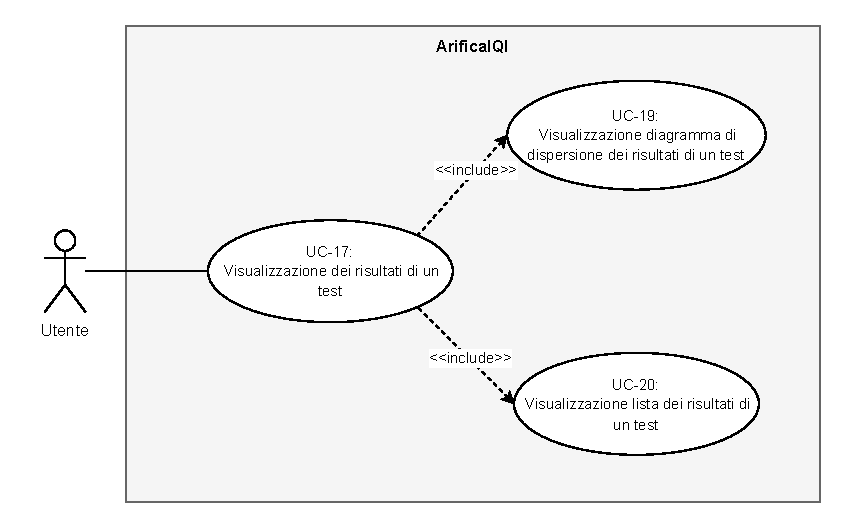
\includegraphics{Sezioni/UseCase/Immagini/UC-17.pdf}
    \caption{Diagramma UC-17.}
\end{figure}

\begin{usecase}{UC-17}{Visualizzazione dei risultati di un test}

    \req{\hyperref[item:RU-6]{RU-6}} 

    \pre{
        \item Il sistema è attivo e funzionante
        \item Sono disponibili i risultati di un test
    }

    \post{
        \item L'utente conosce l'esito del test
    }
    
    \actor{Utente}

    \subactors{}

    \trigger{L'utente deve testare il LLM usando il dataset caricato}
    
    \inc{\hyperref[subsec:UC-19]{UC-19}, \hyperref[subsec:UC-20]{UC-20}}

    \base{}

    \scenario{
        \item \texttt{<<include:UC-19>>}
        \item \texttt{<<include:UC-20>>}
    }

\end{usecase}